\documentclass[11pt]{article}
\usepackage[margin=2.4cm]{geometry}
\usepackage{graphicx,booktabs,float,xcolor,amssymb}
\usepackage[hidelinks]{hyperref}
\usepackage{helvet}\renewcommand{\familydefault}{\sfdefault}
\usepackage{tcolorbox}
\newcommand{\Mw}{M\textsubscript{w}}
\title{\textbf{The 2023-09-08 Al Haouz, Morocco earthquake (\Mw~6.8, us7000kufc):\\
a reproducible MTUQ + WISP validation study of a shallow continental thrust}}
\author{M.-S. Seo\\ \small MTUQ (point-source moment tensor) + WISP (kinematic finite fault); every parameter documented}
\date{13 July 2026}
\begin{document}\maketitle

\begin{abstract}
We determine the point-source moment tensor (MTUQ) and a kinematic finite-fault model (WISP)
of the 2023-09-08 22:11:01 UTC \Mw~6.8 Al Haouz earthquake --- a shallow ($\sim$26~km)
oblique-reverse thrust in the Moroccan High Atlas that killed $\sim$2{,}900 people. Unlike the
mostly-unstudied events we analysed previously, this one has a USGS moment tensor \emph{and}
finite-fault model, so we use it to \emph{validate} the pipeline and to document every data,
frequency-band and processing parameter for reproducibility. Our double-couple moment tensor,
$256/67/65$ (\Mw~6.95), lies 5.1$^\circ$ (Kagan angle) from the USGS W-phase solution; our WISP
finite fault on the steep plane (peak slip 1.46~m at 17--37~km, $\sim$43$\times$38~km) closely
reproduces the USGS model (1.88~m, 25~km, 45$\times$30~km) and prefers the same steep nodal
plane. The study also yields a methodological result that mirrors our deep-event work: for a
\emph{shallow} source the joint body-plus-surface-wave inversion returns a \emph{confidently
wrong} (flipped, normal-faulting) mechanism, because surface waves are dip-slip-indeterminate at
shallow depth (Kanamori \& Given, 1981) and mismatched by 1-D dispersion; the body waves, through
their depth phases, carry the correct dip-slip sense. Inverting body-only recovers the USGS
mechanism.
\end{abstract}

\begin{tcolorbox}[colback=gray!8,colframe=gray!60,title=\textbf{Plain-language summary}]
A magnitude-6.8 earthquake struck the High Atlas mountains south of Marrakesh, on a reverse
(compressional) fault about 26~km deep. Because this event is already well studied, we use it to
\emph{check} our analysis tools against the U.S. Geological Survey's published answers --- and
they agree closely. Along the way we found a trap specific to shallow earthquakes: the
long-period ``surface waves'' cannot tell which way such a fault slipped and gave the
\emph{opposite} (pull-apart) answer; the shorter-period ``body waves'' gave the correct
(push-together) answer. This is the mirror image of what we learned for very deep earthquakes,
where the body waves were the unreliable ones.
\end{tcolorbox}

\section{Event and USGS benchmarks}
The earthquake (31.058$^\circ$N, 8.385$^\circ$W) is an intra-continental oblique-reverse rupture
in the High Atlas. The USGS W-phase moment tensor is $122/29/132$ (shallow SE-dipping) with
conjugate $255/69/69$ (steep NW-dipping), 94\% double couple, centroid 30.5~km; the Mwc (26~km)
and Mwb (24~km) solutions and the 19-km catalogue hypocentre span a genuine \emph{depth debate}.
The USGS finite-fault model adopted the \textbf{steep} plane (strike 251$^\circ$, dip 69$^\circ$),
45$\times$30~km, peak slip 1.88~m, depth 25~km. These are the numbers we reproduce.

\section{Data and parameters (documented for reproducibility)}
\textbf{Determinism.} FDSN data fetching is deterministic in its \emph{parameters} but not across
\emph{time} (data-centre availability changes; transient request failures drop stations). The
reproducible unit is therefore the archived waveforms plus the parameters below: re-running from
the saved SAC files is byte-deterministic, while re-fetching yields a near-identical set. The
inversions are deterministic (MTUQ is an exhaustive grid search; WISP's annealing reproduces to
four decimals). \textbf{Compute} is CPU-only (no GPU): MTUQ parallelises with MPI
(\texttt{mpirun -n 20}); WISP uses OpenMP (Green's functions and annealing) plus a
\texttt{multiprocessing} pool for data processing.

\begin{table}[H]\centering\small
\begin{tabular}{ll}
\toprule
item & value \\
\midrule
WISP data & \texttt{ffm manage acquire -t body} (II, G, IU, GE), $\sim$150 broadband stations \\
MTUQ data & 20 GSN broadband, 31--86$^\circ$, reused from the WISP fetch; response via StationXML \\
 & inventory (output DISP), rotated ZNE$\to$RT \\
MTUQ body band & \textbf{15--40~s} (\texttt{-{}-bwband 15,40,80,8}); 80-s window, $\pm$8~s shifts \\
MTUQ surface band & 50--100~s (shown to \emph{flip} the shallow mechanism; excluded from the solution) \\
MTUQ Green's functions & syngine ak135 (\texttt{ak135f\_2s}) \\
MTUQ grid & DoubleCoupleGridRegular, 40 pts/axis ($\sim$64k orientations $\times$ 5 magnitudes) \\
WISP body filter & 0.006--1.0~Hz, wavelet scales 2--8 \\
WISP surface waves & used (shallow source; above the 125-km surface-wave GF cap) \\
adopted depth & 26~km \\
\bottomrule
\end{tabular}
\end{table}

\begin{figure}[H]\centering
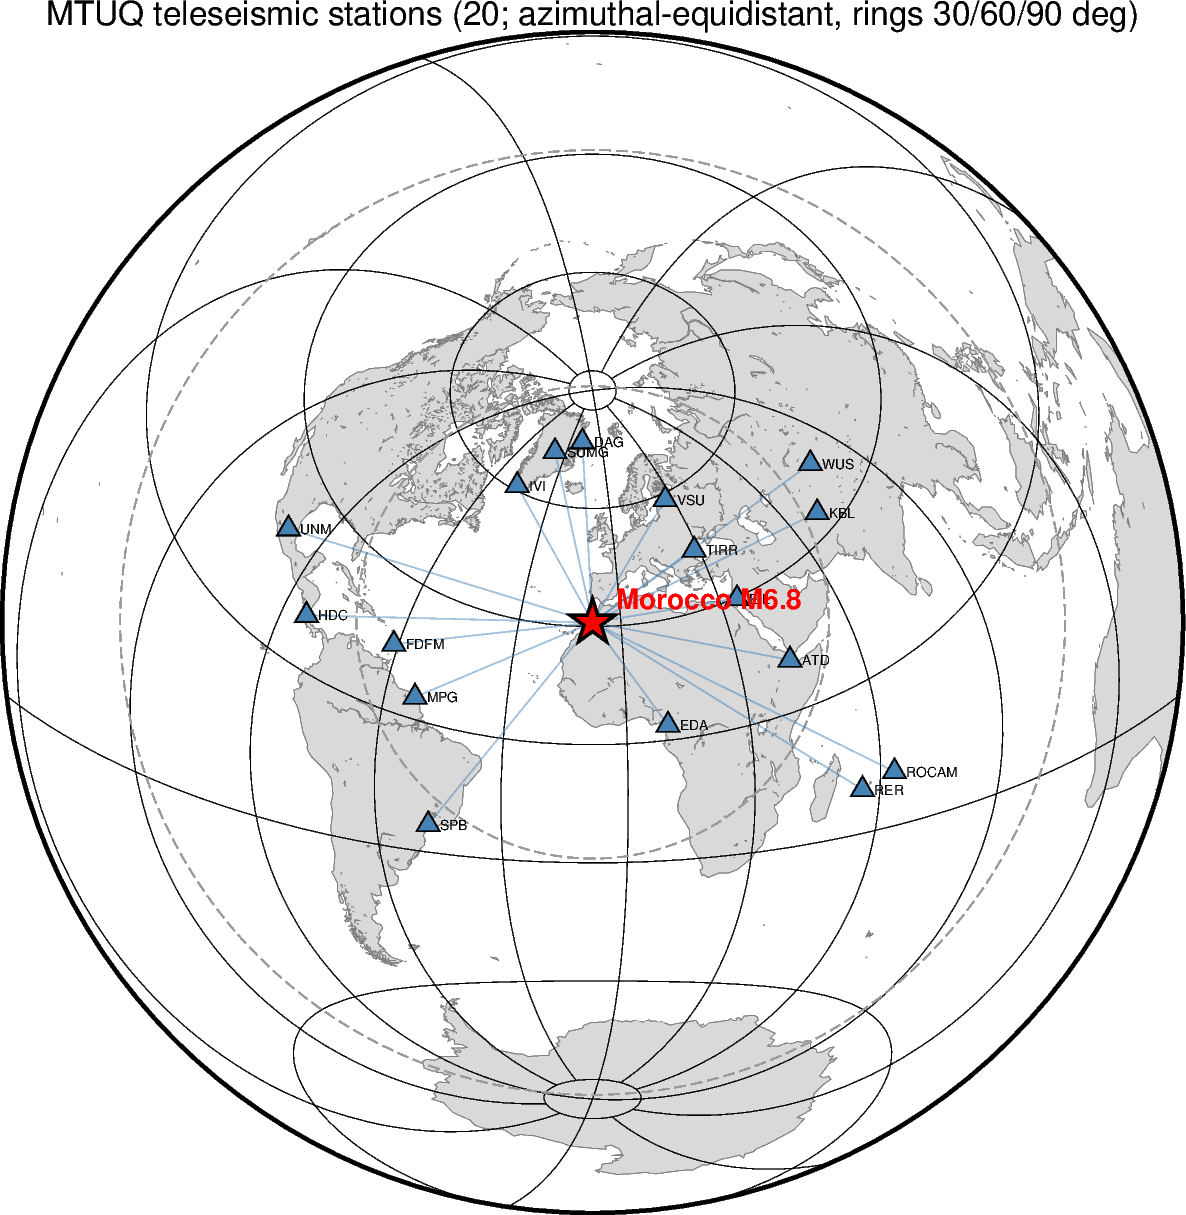
\includegraphics[width=0.72\textwidth]{fig_morocco_stations.png}
\caption{The 20 GSN teleseismic broadband stations used for the moment tensor, on an
azimuthal-equidistant projection centred on the epicentre (rings at 30/60/90$^\circ$).}
\end{figure}

\section{Moment tensor: the shallow-event trap and cure}
Run jointly (body 10--33~s $+$ surface 50--100~s), the DC search converges \emph{confidently} on
a flipped, normal-faulting mechanism $\sim$89$^\circ$ (Kagan) from USGS. The cause is physical:
at shallow depth the vertical dip-slip moment-tensor elements ($M_{rt}$, $M_{rp}$) are weakly
excited at long period --- the Kanamori--Given shallow indeterminacy --- and the surface waves
are additionally mismatched by 1-D dispersion (large time shifts, poor amplitude fit), so they
cannot fix, and actively mislead, the dip-slip sense. The \textbf{body waves}, through their
depth phases, resolve it. We therefore invert \textbf{body-only} (a \texttt{-{}-onlybody} option
added to the runners). This is the mirror image of the deep-event rule, where short-period body
waves fail and the surface/long-period waves are reliable.

\begin{table}[H]\centering\small
\begin{tabular}{lllll}
\toprule
solution & \Mw & strike/dip/rake & Kagan vs USGS Mww & \%DC \\
\midrule
\textbf{DC (adopted)} & 6.95 & \textbf{256/67/65} & \textbf{5.1$^\circ$} & --- \\
full moment tensor & 6.80 & 270/63/63 & 19.1$^\circ$ & 66\% (USGS 94\%) \\
\bottomrule
\end{tabular}
\caption{Body-only MTUQ. The DC solution matches USGS to 5.1$^\circ$; the full MT is destabilised
by the same shallow-source indeterminacy (spurious non-DC, 66\% vs 94\%), which is exactly why
the DC constraint is standard for shallow sources. We adopt the DC solution.}
\end{table}

\begin{figure}[H]\centering
\includegraphics[width=0.42\textwidth]{../../results/mtuq_dc_2023morocco/2023morocco_beachball.png}
\caption{Adopted DC moment tensor (256/67/65) with the teleseismic station distribution ---
the correct oblique-reverse thrust.}
\end{figure}
\begin{figure}[H]\centering
\includegraphics[width=0.92\textwidth,height=0.9\textheight,keepaspectratio]{../../results/mtuq_dc_2023morocco/2023morocco_waveforms.png}
\caption{Body-wave fits of the adopted DC solution (black observed, red synthetic).}
\end{figure}
\begin{figure}[H]\centering
\includegraphics[width=0.92\textwidth,height=0.9\textheight,keepaspectratio]{../../results/mtuq_sota_2023morocco/2023morocco_waveforms.png}
\caption{Body-wave fits of the full moment tensor (270/63/63, 66\% DC), shown for completeness;
the adopted solution is the better-constrained DC.}
\end{figure}

\section{Depth}
The catalogue (19~km), Mwc (26~km), USGS finite fault (25~km) and Mww centroid (30.5~km)
disagree. A joint depth search is unreliable here (the surface-wave flip contaminates it), so we
run a \textbf{body-only} DC+depth search: its global misfit minimum is at $\sim$33~km (a broad
30--34~km trough), independently supporting the \textbf{deeper centroid} ($\sim$30--33~km,
matching the USGS Mww 30.5~km) over the 19-km catalogue hypocentre, with a weaker secondary
minimum near 10--14~km from the depth-phase trade-off. The WISP slip (below) spreads over
17--37~km, consistent with this mid-to-deep-crustal centroid.
\begin{figure}[H]\centering
\includegraphics[width=0.7\textwidth]{../../results/mtuq_bodydepth_morocco/2023morocco_misfit_depth.png}
\caption{Body-only misfit versus source depth (best $\sim$33~km).}
\end{figure}

\section{Finite fault: validation against the USGS model}
We ran WISP \texttt{auto\_model} on both nodal planes of \emph{our own} MTUQ mechanism (internal
consistency: the fault planes come from our moment tensor, not an external CMT). Being shallow,
surface waves are fully used, together with teleseismic P (35 channels) and \textbf{SH} (26 channels) body waves.

\begin{table}[H]\centering\small
\begin{tabular}{llllll}
\toprule
plane & misfit & peak slip & slip depth ($>$15\%) & $L\times W$ & USGS finite fault \\
\midrule
\textbf{steep 256/67 (preferred)} & \textbf{0.1364} & 1.46~m & 17--37~km & 43$\times$38~km & 251/69, 1.88~m, 25~km, 45$\times$30~km \\
shallow 127/25 & 0.1402 & 1.50~m & 11--44~km & 39$\times$38~km & --- \\
\bottomrule
\end{tabular}
\caption{The steep plane is preferred (agreeing with the USGS choice), and its slip model closely
reproduces the USGS finite fault in amplitude, depth and dimension. As for the Chile events the
teleseismic \emph{fit} difference between planes is small; the steep-plane preference is
corroborated by USGS aftershocks and InSAR.}
\end{table}

\begin{figure}[H]\centering
\includegraphics[width=0.9\textwidth]{../../event_2023_morocco_mtuq/20230908221101/ffm.0/NP2/plots/SlipDist_plane0_5s.png}
\caption{Preferred (steep-plane) slip model. Star: hypocentre; contours: rupture front every 5~s;
arrows: slip direction (reverse). Peak 1.46~m, slip at 17--37~km depth.}
\end{figure}
\begin{figure}[H]\centering
\includegraphics[width=0.55\textwidth]{../../event_2023_morocco_mtuq/20230908221101/ffm.0/NP2/plots/MomentRate.png}
\caption{Moment-rate function (steep plane).}
\end{figure}
\begin{figure}[H]\centering
\includegraphics[width=0.92\textwidth]{../../event_2023_morocco_mtuq/20230908221101/ffm.0/NP2/plots/P_body_waves.png}
\caption{WISP P-wave fits (steep plane).}
\end{figure}
\begin{figure}[H]\centering
\includegraphics[width=0.92\textwidth]{../../event_2023_morocco_mtuq/20230908221101/ffm.0/NP2/plots/SH_body_waves.png}
\caption{WISP SH-wave fits (steep plane): teleseismic SH (transverse, 26 channels) are used
alongside the 35 P channels.}
\end{figure}
\begin{figure}[H]\centering
\includegraphics[width=0.92\textwidth]{../../event_2023_morocco_mtuq/20230908221101/ffm.0/NP2/plots/Rayleigh_surf_waves.png}
\caption{WISP Rayleigh-wave fits (steep plane).}
\end{figure}

\section{Summary}
\begin{enumerate}
\item The pipeline \textbf{reproduces the USGS moment tensor to 5.1$^\circ$ and the USGS
finite-fault model} (slip amplitude, depth, dimensions, preferred plane) for this well-studied
event --- a clean end-to-end validation across a new tectonic regime (shallow continental thrust).
\item \textbf{Shallow-event rule:} invert \emph{body waves} for the mechanism; surface waves are
dip-slip-indeterminate at shallow depth and flip the solution. Mirror of the deep-event rule.
\item \textbf{Use the DC constraint} for shallow sources --- the full MT is destabilised by the
same indeterminacy (66\% vs USGS 94\% DC).
\item Every parameter is tabulated; the analysis re-runs deterministically from the archived
waveforms. Pipeline is CPU-parallel (MPI $+$ OpenMP), no GPU.
\end{enumerate}
\end{document}
